\chapter{Practical Applications: Training on a Specific Task}

\section{Datasets}

In the last few years, the most popular dataset for modern object detectors was the Common Objects in Context (COCO) dataset~\footnote{\url{}} \textbf{(source? + insert paper citation)}. The publications discussed in the previous chapters have all been evaluated on the COCO~2017 dataset. It is also used for segmentation, but the object detection dataset in itself contains annotations of 80 classes, so the best models learn fairly general representations of many visual features from objects.

However, in this work I am going to specialise my models of choice for vehicle detection. Theoretically, taking the COCO dataset and stripping all but 2 of its classes, the \textit{car} and \textit{truck} classes provides a vehicular dataset, and eventually chosing images that contain none of the above as \textit{hard negatives} should work satisfactory. However, during the research I have found two vehicle-centered, public datasets available: the kitti dataset, and the UA-DETRAC dataset.

I conducted initial data exploration on the COCO dataset with the FiftyOne tool (launching an application session from a Python shell as described in their tutorials), as seen in figure~\ref{fig:fiftyone-car-truck}.

% \begin{center}
%     \captionof{figure}{Exploring the train split of the MS COCO 2017 dataset in the FiftyOne tool. There are 43867 instances of labeled cars and 9973 instances of labeled trucks, with 14714 images containing either of them.}
%     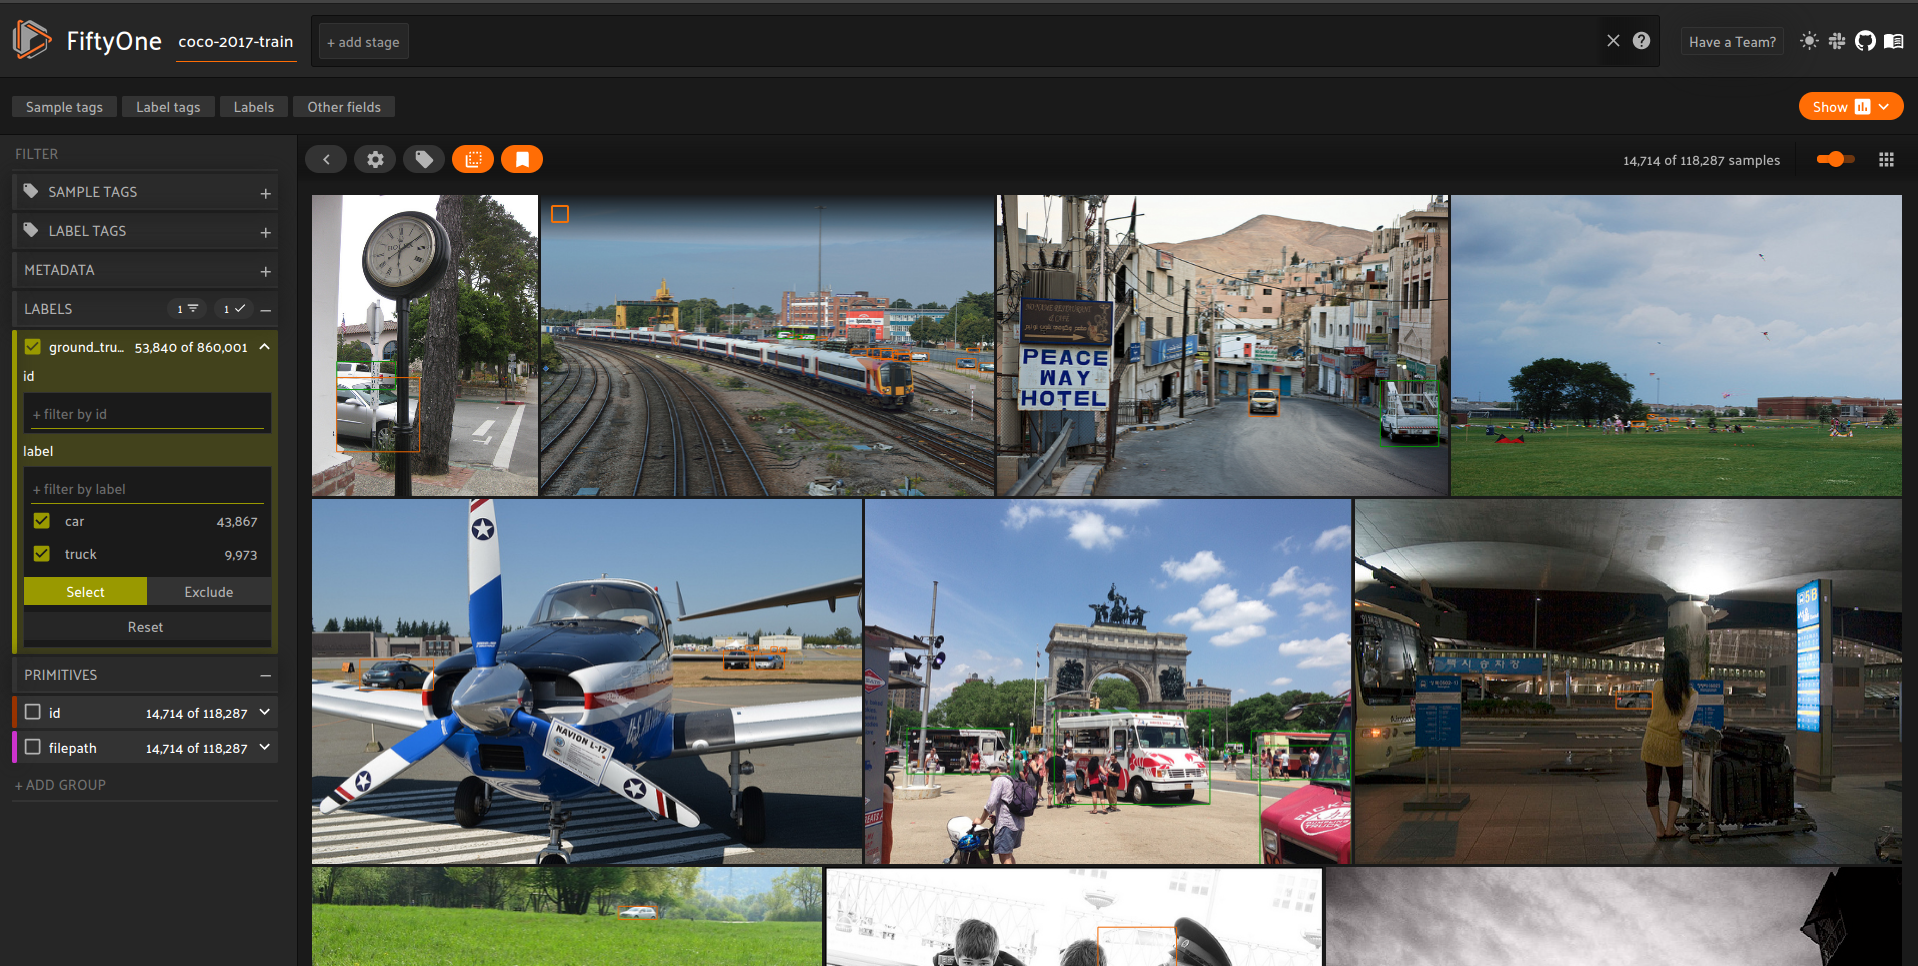
\includegraphics[width=\textwidth]{figures/fiftyone-coco-car-truck.png}
%     \label{fig:fiftyone-car-truck}
% \end{center}

\begin{figure}[h]
    \captionsetup{width=\textwidth}
    \caption{Exploring the train split of the MS COCO 2017 dataset in the FiftyOne tool. There are 43867 instances of labeled cars and 9973 instances of labeled trucks, with 14714 images containing either of them.}
    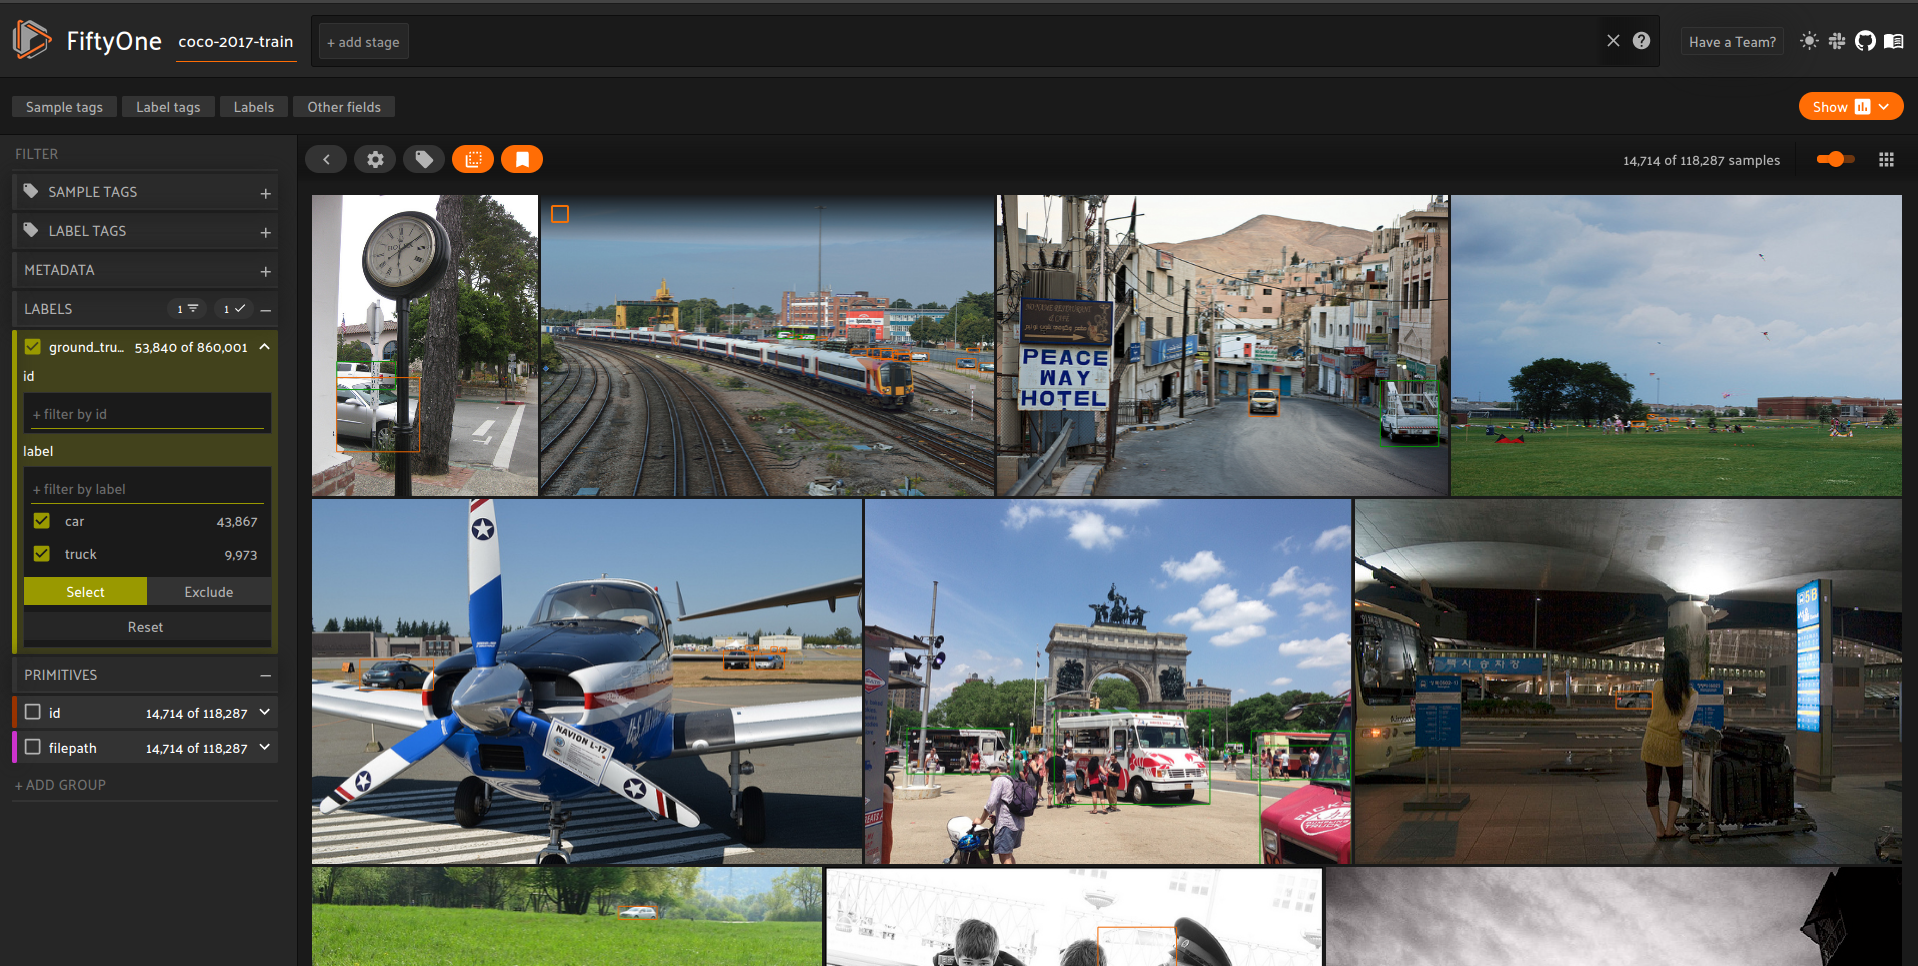
\includegraphics[width=\textwidth]{figures/fiftyone-coco-car-truck.png}\label{fig:fiftyone-car-truck}
\end{figure}

\begin{figure}[h]
    \captionsetup{width=\textwidth}
    \caption{Some difficult examples: objects in overexposed regions of the image, crowd labels consising of very small (e.g aerial) images of cars (orange) and trucks(green)}
    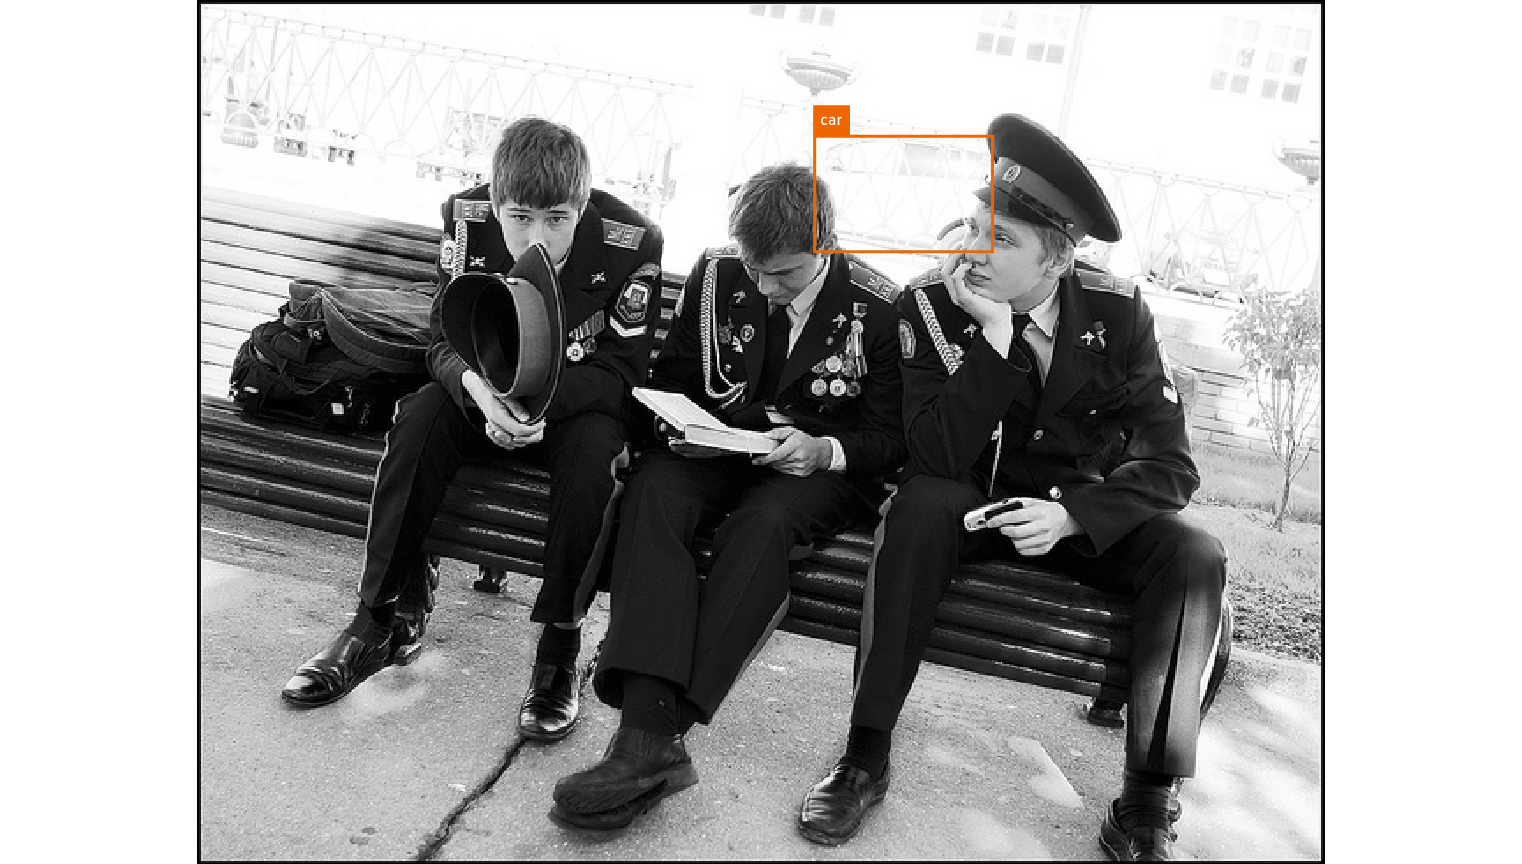
\includegraphics[width=.49\textwidth]{figures/car-overexposed.png}
    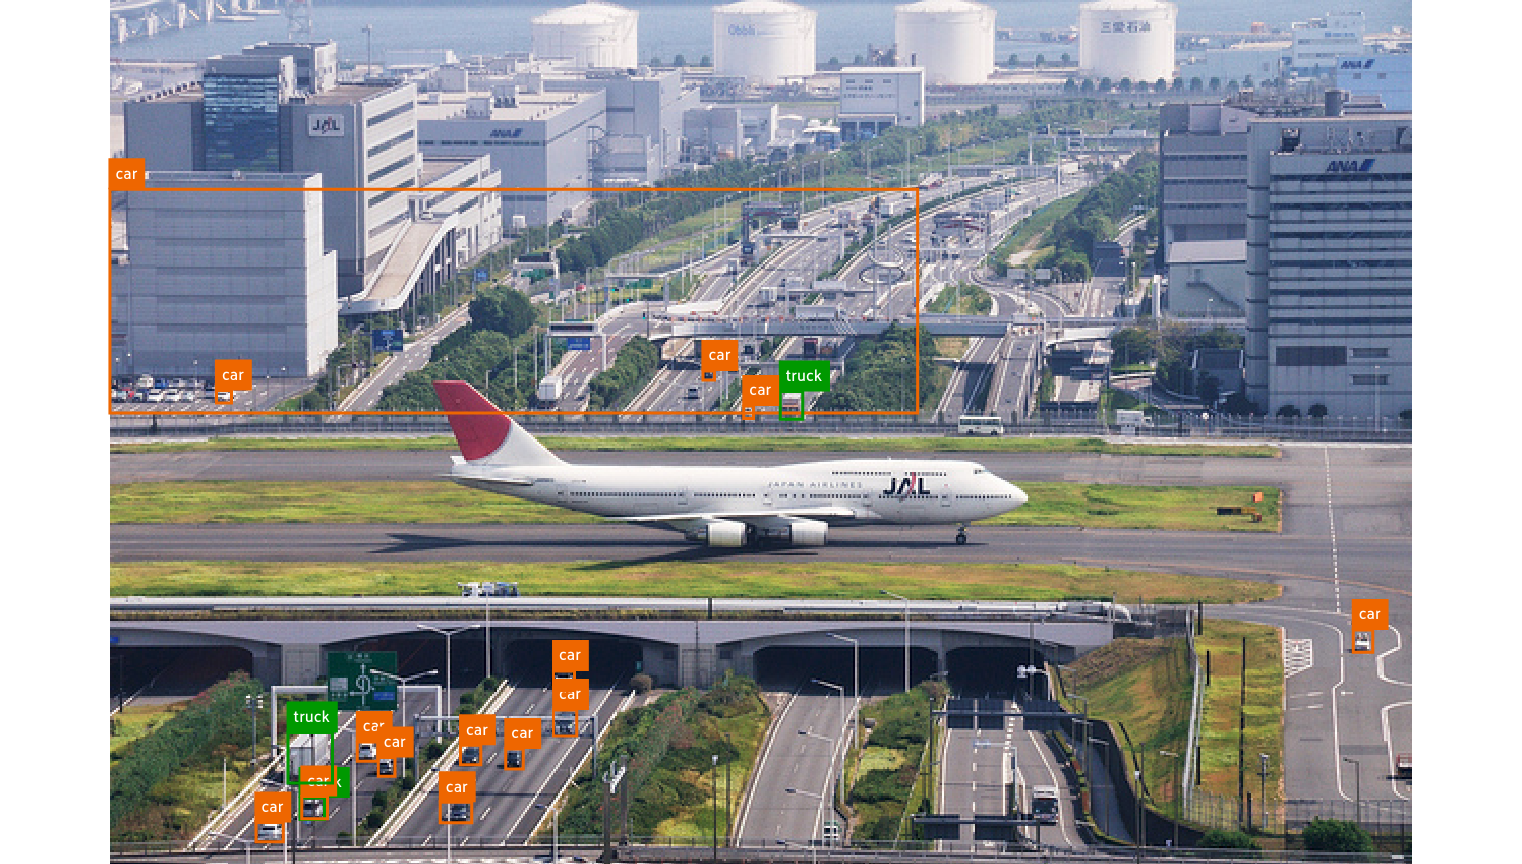
\includegraphics[width=.49\textwidth]{figures/car-truck-small-crowd.png}\\
    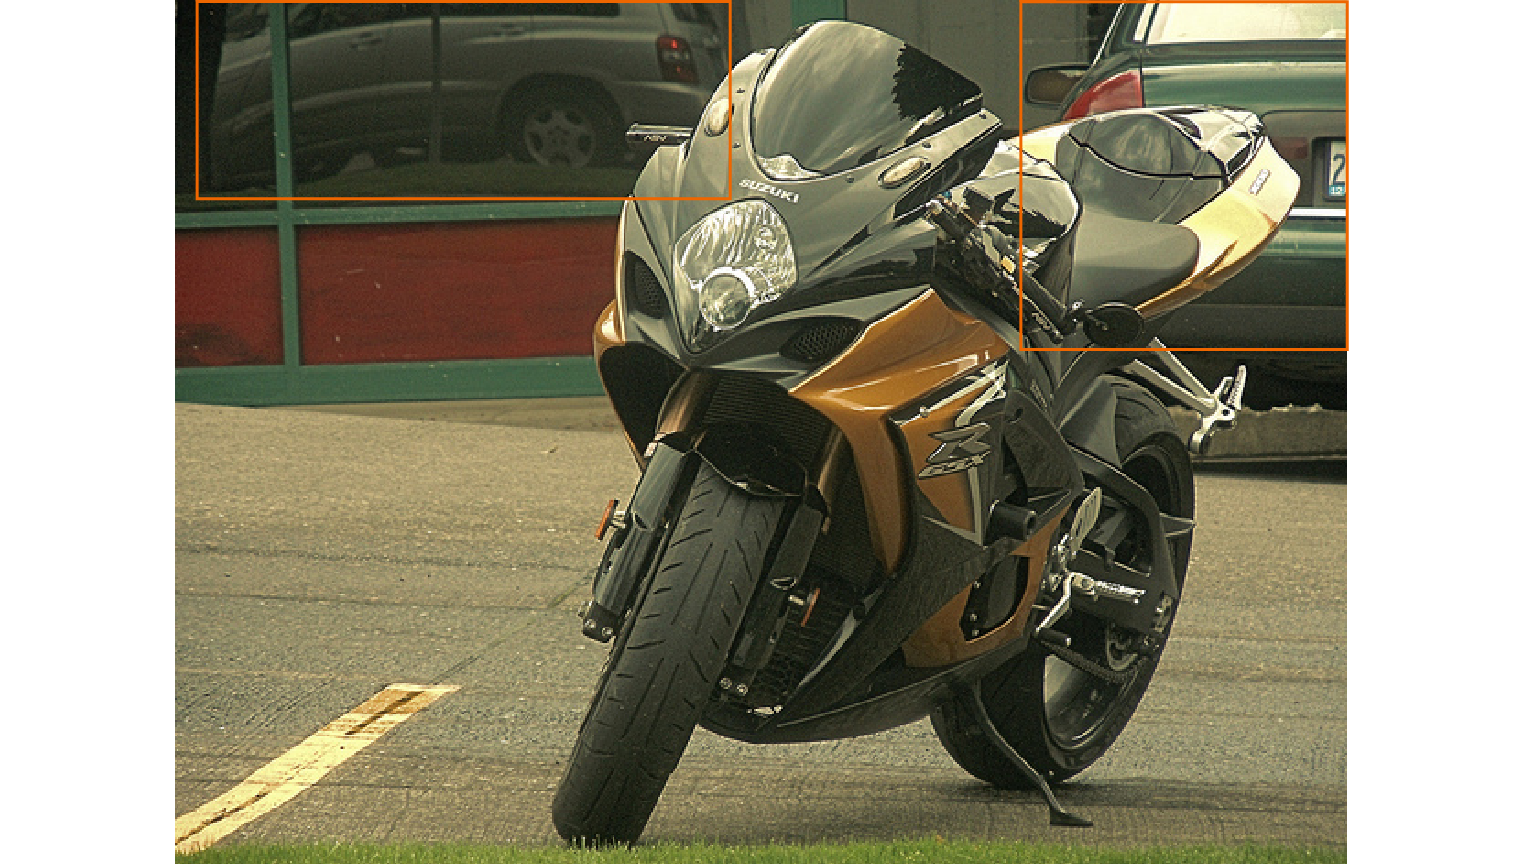
\includegraphics[width=.49\textwidth]{figures/car-reflection-partial.png}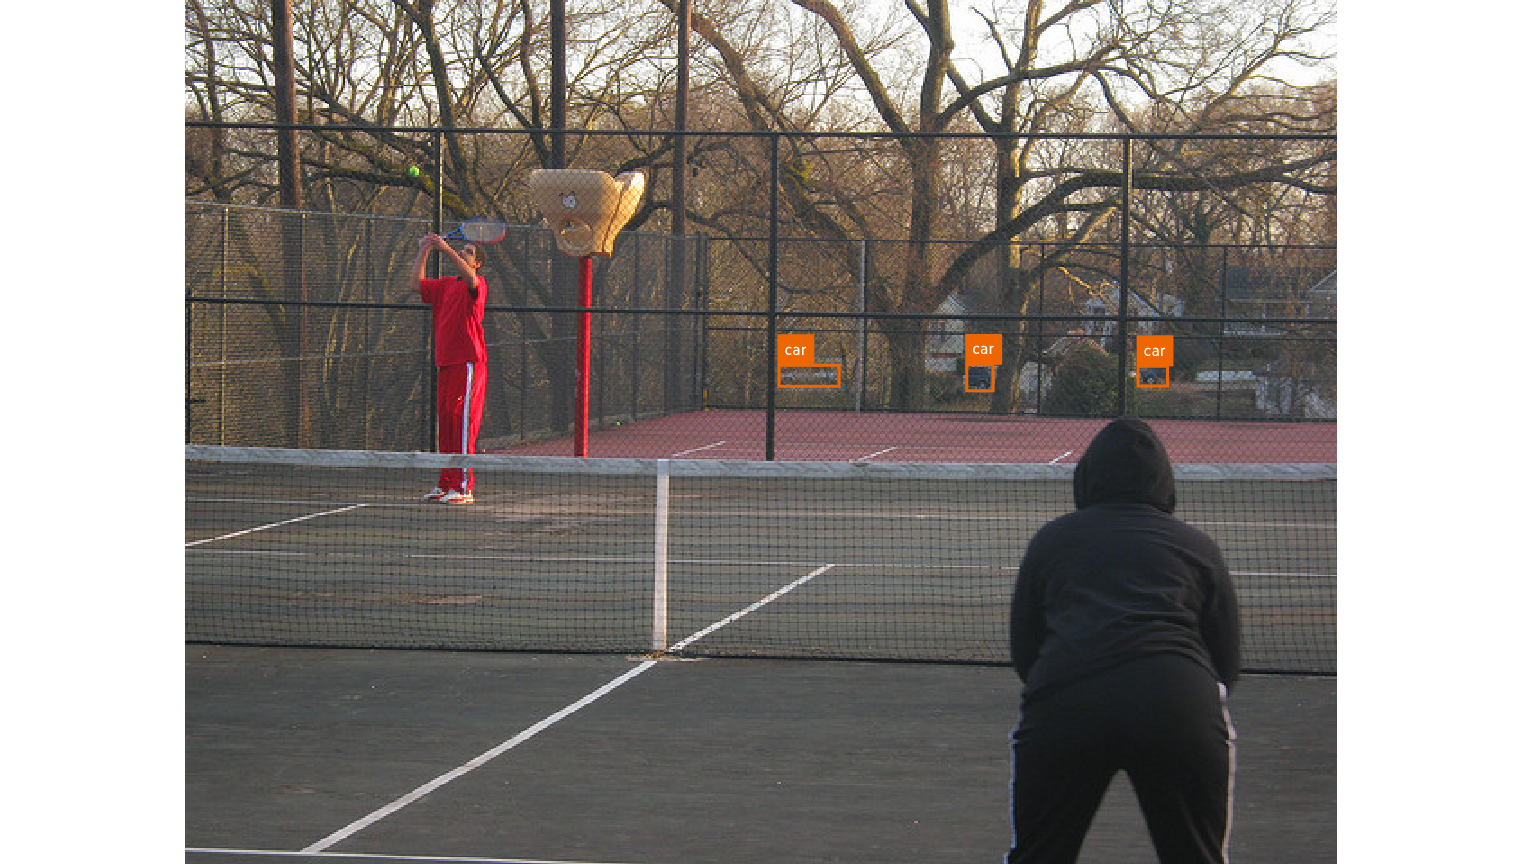
\includegraphics[width=.49\textwidth]{figures/car-obscure.png}\\
\end{figure}

% \subsection{kitti}




% \section{Training via Transfer Learning}

% \subsection{DETR}
